\documentclass[a4paper]{article}
\usepackage{listings}
\usepackage{xcolor}
\usepackage {fontspec}
\usepackage {multicap}
\usepackage{fancyhdr}
\pagestyle{fancy}
\setromanfont{Lantinghei SC Extralight}
\setmonofont{Courier New}
\XeTeXlinebreaklocale ``zh''
\XeTeXlinebreakskip = 0pt plus 1pt
\textheight = 650pt
\lstset{
	%行号
   numbers=left,
  %背景框
   framexleftmargin=10mm,
   frame=none,
   %背景色
   %backgroundcolor=\color[rgb]{1,1,0.76},
   backgroundcolor=\color[RGB]{245,245,244},
   %样式
   keywordstyle=\bf\color{blue},
   identifierstyle=\bf,
   numberstyle=\tiny,
   numberstyle=\color[RGB]{0,192,192},
   commentstyle=\it\color[RGB]{0,96,96},
   stringstyle=\rmfamily\slshape\color[RGB]{128,0,0},
   %显示空格
   showstringspaces=false
 }

\begin{document}
\title{实验报告 实验九}
\author{姓名:王钦\quad 学号:13349112\quad 班级:计科二班}
\date{}

\maketitle
\section*{ 实验目的}
\hangindent=4em \hangafter=-10{
1. 学习FAT12文件系统组织方法,掌握其实现方法。\\
2. 利用FAT12文件系统实现原型操作系统的自身引导。\\
3. 扩展MyOS,利用FAT12文件系统实现加载用户程序。\\
}
\section*{ 实验内容}
\hangindent=4em \hangafter=-10{
  在实验五或更后的原型基础上,进化你的原型操作系统,原型保留原有特征的基础上,设计满足下列要求的新原型操作系统:\\
  (1)实现1.44MB软盘映像文件上的FAT12格式。\\
  (2)内核执行体以COM格式文件形式存放在映像的FAT12文件系统中,修改引导程序实现内核的加载.\\
  (3)将所有测试的用户程序放在在映像文件中的FAT12文件系统中,修改内核,实现从文件系统加载用户程序。\\
}

\section*{ 实验平台}
\hangindent=4em \hangafter=-10{
  xxd+dd+gcc+ld+nasm+Linux+vim\\
  实验报告编辑:Latex
}

\section*{ 算法流程图}
\hangindent=4em \hangafter=-10{
  \begin{center} 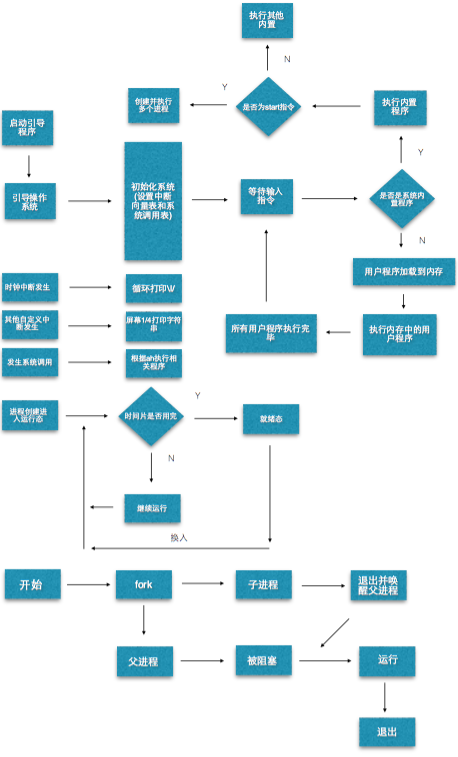
\includegraphics[scale=0.5]{Illustrations/flow0.png} \mfcaption{other}\end{center}
  \begin{center} 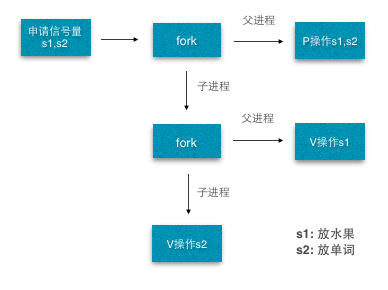
\includegraphics[scale=0.5]{Illustrations/flow1.png} \mfcaption{process}\end{center}
}

\section*{ 功能一览}
\hangindent=4em \hangafter=-50{
	{\large 1. 系统内置功能:}\\
		\indent \verb| terminal|,装载内核shell,为用户提供一个与操作系统交互的工具,开机后自动进入,以下所有功能都在terminal中交互\\
		\indent \verb| clear|, 清除当前屏幕所有字符,刷新屏幕\\
		\indent \verb| help|, 显示系统帮助信息\\
		\indent \verb| python |, python 扩展,类似python命令行工具,可以使用这个工具输入计算表达式返回计算结果,目前只支持加法减法\\
		\indent \verb| start|, 开始创建并执行四个进程并且每秒18.2次的调度,分别在屏幕\verb|1/4|处打印一些个性化信息( 不同配置的虚拟机动画速度不一样,建议使用bochs测试)\\\\
	{\large 2. 用户程序:}\\
		\indent \verb| run |,软盘中含有两个用户程序,输入\verb|run 12|,可分别执行两个用户程序,当然也可以通过改变执行序列来改变执行的顺序\\\\
	{\large 3. 自定义中断:}\\
		\indent 时钟中断:通过PTR每秒发出18.2次的信号来从8592芯片的RT0引脚发出终端号\verb|int 08h|来触发的用户时钟软中断\verb| int 1ch|,实现在\verb|terminal|的右下角
	  一个横杠在转动.\\
		\indent 另外有自定义中断\verb|int 33h,int 34h,int 35h,int 36h|分别在屏幕四分之一的位置打印个性化信息\\\\
	{\large 4. 进程调度:}\\
		\indent 软盘中共存放了用于展示进程调度的六个应用程序,其中一个应用程序为监听用户键盘事件然后退出多进程调度状态回到\verb| terminal|每个应用程序分别代表一个进程。开启装载进程并进行进程调度由\verb|1|中系统内置功能的\verb| start|指令激活。\\
		\\
	{\large 5. 进程\verb|fork,wait,exit|:}\\
		\indent 具体使用在第六个进程中,执行\verb|start|后即可看到包括第六个进程在内全部进程执行的结果。\\\\
	{\large 6. 使用信号量解决进程间的同步:}\\
		\indent 具体使用在第六个进程中,执行\verb|start|后即可看到包括第六个进程在内全部进程执行的结果。\\\\
	{\large 7. 文件系统}\\
		\indent 硬盘内容的加载均使用unix文件系统的形式管理,执行\verb|ls| 命令可以查看用户区有哪些文件\\\\
}

\section*{ 实验步骤及效果图}
\hangindent=4em \hangafter=-50{
	\begin{enumerate}
		\item 运行\verb| ls|命令,查看所有用户程序文件
		\begin{center} 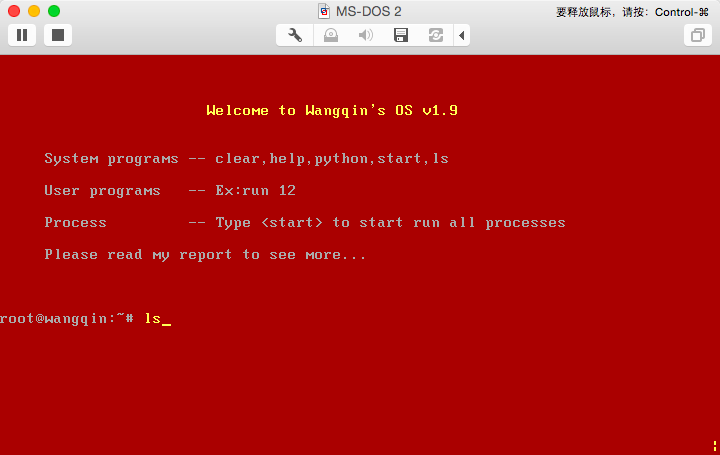
\includegraphics[scale=0.4]{Illustrations/ls.png} \mfcaption{ls}\end{center}
		\begin{center} 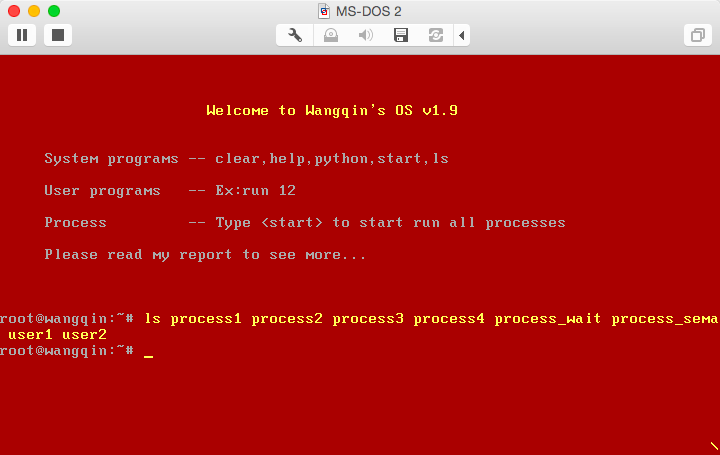
\includegraphics[scale=0.4]{Illustrations/ls_resu.png} \mfcaption{ls\_result}\end{center}
		\item 运行\verb| run user1|命令,运行第一个用户程序
		\begin{center} 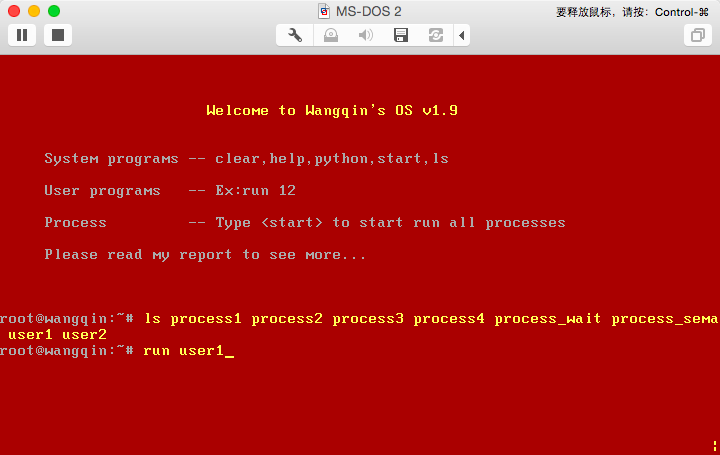
\includegraphics[scale=0.4]{Illustrations/run.png} \mfcaption{run}\end{center}
		\begin{center} 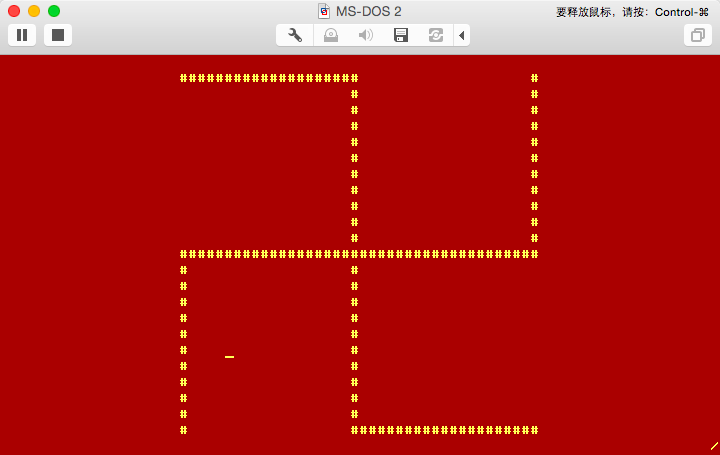
\includegraphics[scale=0.4]{Illustrations/run_resu.png} \mfcaption{run\_result}\end{center}
	\end{enumerate}
}
\section*{ 内存和软盘存储管理}
\hangindent=4em \hangafter=-50{
1. 引导程序加载到内存0x7c00处运行\\
2. 引导程序将操作系统加载到0x7e00处运行\\
3. 操作系统讲用户程序加载到0x1000处运行\\
4. 软盘第0个柱面的第一个扇区存储操作系统引导程序\\
5. 软盘第0个柱面剩下所有扇区2~36扇区存储操作系统内核\\
6. 软盘第\verb|1,2,3,4,5,6|柱面分别存储六个进程代码\\
7. 软盘第\verb|7,8|柱面分别存储两个用户程序的程序代码\\\\
{\large 栈结构}\\
	\indent 内核栈:从内存的\verb| 0xffff|开始向下扩展\\
	\indent 用户栈:从内存的\verb| 0x1000|开始向下扩展\\
	\indent 进程栈:第i个进程对应的进程栈从内存的\verb| i*0x800|开始向下扩展\\
	\indent 第六个进程之后会有点特殊每次进程栈会加0x1000(主要为了保障fork后的进程有足够大的栈),例如第六个是0x3000,
	第七个是0x4000,第八个是0x5000...\\\\
更多细节信息请阅读我的Makefile文件
}
\section*{ 系统目录结构}
\hangindent=4em \hangafter=-50{
{\scriptsize
  \setmonofont{Lantinghei SC Extralight}
\begin{verbatim}
.
├── Makefile							makefile 文件
├── README
├── bochsrc                             bochs配置文件
├── boot.asm                            引导程序
├── disk.img							镜像文件
├── kernel                              目录中存放内核相关代码
│   ├── fcb.h							文件控制模块
│   ├── os.asm                           主要为os.c提供函数实现.
│   ├── os.c                            为内核主要控制模块
│   ├── os.h                            主要为os.c提供函数实现.
│   ├── os_syscall.asm                  系统调用相关代码
│   ├── osclib.c                        为osclib.c提供更底层的函数封装
│   ├── oslib.asm                       初始化系统调用和设置系统调用相关模块
│   ├── pcb.h							进程控制模块
│   ├── process.c                       进程调度创建以及信号量相关代码
│   ├── terminal.c                      装载shell的工具
│   └── terminal.h
├── muti_process.h                      fork,wait,wakeup,printf等声明实现
├── osclib_share.c                      内核和用户的共享库(使用户程序体积减少)。
├── oslib_share.asm                     内核和用户的共享库(使用户程序体积减少)。
├── process1.asm                        第一个进程
├── process2.asm                        第二个进程
├── process3.asm                        ..
├── process4.asm                        ..
├── process_semaphore.c                 father's gifts 进程(信号量解决)
├── process_wait_key.asm                监听退出进程
├── python_extension.c                  Python扩展
├── report                              实验报告目录
│   ├── Illustrations                   插图
│   │   └── flow.png
│   └── report.tex						Latex文件
├── snapshot.txt
├── usr1.asm							用户程序1
├── usr2.asm							\ldots
└── usrlib.asm							用户程序专用汇编库(不与内核共享)

3 directories, 31 files
\end{verbatim}}
}

\setmonofont{Courier New}

\section*{ 主要函数模块}
\hangindent=4em \hangafter=-50{
	\begin{enumerate}
\item \verb|fcb|,文件控制模块,记录着文件的属性和一些信息的一组数据,\verb|name|文件名,\verb|f_num|文件编号,\verb|f_size|文件大小,\verb|f_addr|文件地址,\verb|f_toMem|文件加载到内存的地址.
{\scriptsize\begin{lstlisting}[language={C}]
struct fcb{
 const char *name;
 char f_num;
 char f_size;
 char f_addr;		//block num
 int f_toMem;		//
};
struct fcb FCB_array[ file_sum];
 		\end{lstlisting}}
	\item \verb|loadfile|,将文件加载到指定内存地址
{\scriptsize\begin{lstlisting}[language={C}]
	load_user:
	;load os to mem

	mov ax,cs
	mov es,ax

	mov cx,1;

	;next_lu:


	mov dx,bp	;backup
	mov bp,sp
	mov ch,[ bp+4]		; 柱面/磁道  every zhumian  has one user program 37~72  73~108 109~144		ch = 7~8 is user
	mov bx,[ bp+8] ;add to 0x100 mem
	
	mov bp,dx

	mov dl,0		; 软盘
	mov dh,0		; 磁头:正面

	xor ax,ax
	mov es,ax ;made es zero,ex:bx is addr of mem 
	mov ax,0215h	;count 

	int 13h
	;cmp ch,6
	;je sixun
	;jmp nextaa
	;sixun:
	;jmp $
	;nextaa:

ret

\end{lstlisting}}
\item 一些变量说明
{\scriptsize\begin{lstlisting}[language={C}]

BaseOfLoader			equ	1000h	    ; 根目录 被加载到的位置 ----  段地址
OffsetOfLoader	        equ	4000h	    ; 根目录 被加载到的位置 ---- 偏移地址
RootDirSectors	        equ	14		    ; 根目录占用的扇区数
SectorNoOfRootDirectory	equ	19	        ; 根目录区的首扇区号
SectorNoOfFAT1	        equ	1		    ; FAT#1的首扇区号 = BPB_RsvdSecCnt
DeltaSectorNo		    equ	17		    ; DeltaSectorNo = BPB_RsvdSecCnt + 
; (BPB_NumFATs * FATSz) - 2 = 1 + (2*9) -2 = 17
; 文件的开始扇区号 = 目录条目中的开始扇区号 
; + 根目录占用扇区数目 + DeltaSectorNo

wRootDirSizeForLoop	    dw	RootDirSectors	; 根目录区剩余扇区数
; 初始化为14,在循环中会递减至零
wSectorNo				dw	0           ; 当前扇区号,初始化为0,在循环中会递增
bOdd					db	0			; 奇数还是偶数FAT项
filename                dw  0           ; 文件名指针
baseAddress             dw  0           ; 文件加载段地址
offsetAddress           dw  0           ; 文件加载偏移地址

BPB_BytsPerSec			dw 512          ; 每扇区字节数
BPB_SecPerTrk	        dw 18	        ; 每磁道扇区数
BS_DrvNum		        db 0	        ; 中断 13 的驱动器号(软盘
\end{lstlisting}}
 \end{enumerate}
}
\section*{ 实验心得及仍需改进之处}
\hangindent=4em \hangafter=-50{
	{\large 实验心得:}\\\\
	\indent 本次实验主要是加了文件系统功能使软盘中扇区存放数据和读取到内存的时候按照文件系统的格式实现,由于实验一直在实模式下进行,我的操作系统代码量太过于庞大加载到内存的时候超过了0xb400(0x7e00~0xb400),很奇怪的是代码一超过0xb400就会出一些奇怪的错误。所以我把之前实验要求的几个系统内置功能\verb|time,date,asc|删掉了,还有我自己个性化设置的查看帮助信息的man命令,这样减少了很多代码,操作系统也恢复到了正常状态,仍然不知道这个原因是什么,操作系统实验已经快结束了,可能实验就做到这里了。同时也很怀念调试实验晚上9点吃早餐的那段时间。这门课也是这学期花费精力和时间最多但学分最低却学到内容最多的一门课。至于上面提到的那个问题只能等到以后有时间了再去看了,期末临近实在难抽出时间和精力了。
	\\
\\\\
	{\large 实验仍需改进之处:}\\\\
	\indent 仍需完善细节,比如说\verb|python|的命令行工具加入乘法,除法完全是几行代码的问题\\
	\indent 可以考虑将用户程序做成\verb|elf|格式,动态链接系统的代码库。目前的情况是用户程序自己带着一份和操作系统一样的代码库,分别联合编译\\
	\indent 精简操作系统代码,减少冗余代码\\
	\indent 调度算法和进程控制模块的存储有待优化,使用链表来实现pcb\\
	\indent 信号量池可以考虑使用链表进行存储,此外\verb|fruit_disk|,存在一个互斥的问题,当父亲在改写\verb|fruit_disk=0|的时候,儿子进程可能正在放水果,导致两个进程
	对同一变量进行改写,这个问题通过多申请一个信号量很容易可以解决。\\
}
\end{document}
